\documentclass[a4paper,10pt]{article}
\usepackage[utf8]{inputenc}
\usepackage{amsmath}
\usepackage{graphicx}

%opening
\title{ICE Model - Analytic Solution For Loaded Membrane }
\author{Anupam Prasad Vedurmudi}
\date{}
\begin{document}

\section{Loaded Membrane}
\subsection{Loaded String Analogy}
As an example of an extended vibrating object coupled to a rigid body we consider
a vibrating string attached to a rigid rod of mass $M_R$ at one end. The other ends of both 
the rod and the string are fixed and the rod can rotate about the axis through this
end normal to the plane. The advantage of this system is that, under some reasonable physical
assumptions, it can be solved exactly.
\begin{figure}[htb]
\centering
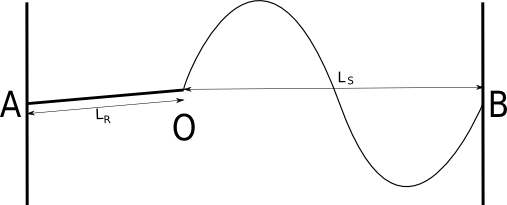
\includegraphics[width=9.5cm]{loadedstring.png}
\caption{String Attached to a Rod of Finite Mass}
\label{loadedstring}
\end{figure}

In the above figure, we have a rigid rod of length $L_R$ attached to a string of length
$L_S$ (at rest). For small vibration amplitudes, we can ignore the changes in the length of
the rod. This means that the end corresponding to the point \textbf{O} moves along a straight line.
\subsubsection{Modes of the Free String}
The equation of motion of a freely vibrating string is given by,
\begin{equation}\label{freestring}
 \frac{\partial^2 z}{\partial t^2} = c_S^2 \frac{\partial^2 z}{\partial x^2}
\end{equation}
Where, $z(x,t)$ is the displacement of the string at time $t$ and at the position $x$. \textbf{O} corresponds
to $x=0$ and \textbf{B} to $x=L_S$. $c_S$ is the propagation speed of transverse waves on the string. It
is given in terms of the string tension, $T$ and total mass, $m_S$ as,
\begin{equation}
 c_S=\sqrt{\frac{TL_S}{m_S}}
\end{equation}
The reason for writing the above expression in this form is that the boundary condition at \textbf{O},
which in turn gives us a discretization condition for the modes can be written in terms of the ratio of
the rod mass and string mass. Otherwise, it is traditionally written in terms of the mass per unit length as, 
$\sqrt{\frac{T}{\lambda}}$.

A specific solution to \eqref{freestring} is found by using separation of variables to be,
\begin{align}
 z(x,t)&=\left(Ae^{jkx}+Be^{-jkx}\right)e^{j\omega t}\\
 \omega&=ck\nonumber
\end{align}
For any $k$. Applying the boundary condition $z(L_S,t)=0$ gives us,
\begin{equation}
 z(x,t)=\sin(k(L_S-x))e^{j\omega t}
\end{equation}
Where we've ignored the coefficient $A$.
\begin{figure}[htb]
\centering
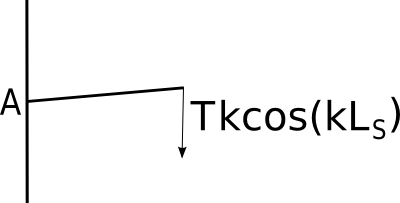
\includegraphics[width=6.5cm,height=3cm]{loadedstring_rod.png}
\caption{Motion of the Rod}
\label{loadedstring_rod}
\end{figure}

\section{Modelling the Loaded Membrane}
We consider a tympanic membrane of radius $a$ with the extra-columellar footplate situated
between $0<\phi<\beta$ and $2\pi-\beta\leq\phi\leq 2\pi$ (or equivalently between
$-\beta<\phi<\beta$). The attached extracolummelar footplate is modelled by 
the following set of equations,
\begin{equation}\label{extracollumela1}
 u_{0/L}(r,\phi,t) = \begin{cases} D_{0/L}\left(1-\frac{r\cos \phi}{a\cos \beta}\right) &\mbox{if } 0\leq r <a\cos \beta/\cos \phi \\
0 & \mbox{if } a\cos \beta/\cos \phi\leq r\leq a \end{cases} 
\end{equation}
where, $\phi$ is in the region mentioned above. The above equations model the
extracollumela as a triangular plate. The model is described in figure \ref{extracolumellafig1} - The triangle
OAB hatches about the line AB and the striped section is rigid. The subscripts $0$ and $L$ denote the ipsi-lateral and contra-lateral 
membranes respectively. The coefficients $D_{0/L}$ will be determined later.
\begin{figure}[htb]
\centering
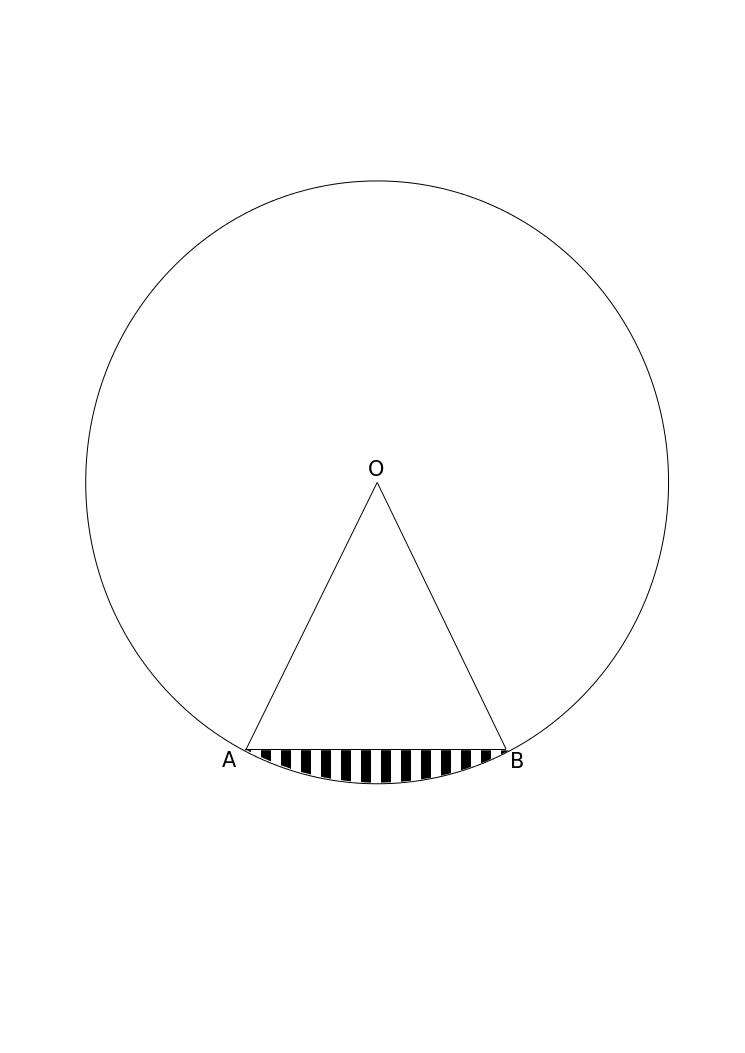
\includegraphics[width=4.5cm]{extracolumella.png}
\caption{Loaded Membrane with Extracolumella situated in the sector OAB}
\label{extracolumellafig1}
\end{figure}
This also requires the membrane to have the same
displacement for a given radius at the angles $\beta$ and $2\pi-\beta$.

\subsection{Infinite Mass Extracolumella}
Analytically solving the system for a moving extracolumella is intractable. Hence, as an approximation,
we assume that the Extracolumella has infinite mass, i.e., it remains stationary. This approximation gives
us the advantage that the motion of the membrane is given as a linear combination of a new set of orthogonal
modes, 

\begin{equation}\label{newmembranemodes}
 f_{mn}(r,\phi)=sin[\mu (\phi-\beta)]J_\mu(k_{\mu n}r)
\end{equation}
where $\mu=\frac{m\pi}{2(\pi-\beta)}$. This value arises because of the new membrane boundary condition
which requires the membrane displacement to go to zero at $\phi=\beta,2\pi-\beta$. We also make note of
the fact that $\int dS f_{mn}(r,\phi)=0$ for even $m$. This means that, analogous to the unloaded
membrane, a uniform periodic pressure only excites the $m$-odd modes. The difference here is that the
these modes are no longer circularly symmetric and their eigenfrequencies are more closely spaced
than those of the unloaded circular membrane.
% \begin{equation}\label{membranegeneralnew}
% u_{0/L}(r,\phi,t)=\sum_{m,n}C^{0/L}_{mn}\cos (m\phi)J_m(\mu_{mn}r)e^{j\omega t}
% \end{equation}
% 
% \subsubsection{Orthogonality}
% We define $f_{mn}(r,\phi)=\cos (m\phi)J_m(\mu_{mn}r)$. These modes satisy the orthogonality condition,
% \begin{equation}\label{orthogonality1}
%  \int dS f_{mn}f_{kl}=\delta_{m,k}\delta_{n,l}\frac{\pi}{2} J^2_{m+1}(\mu_{mn}a)
% \end{equation}
% Where, $dS=rdrd\phi$. This condition relies on the orthogonality of $J_m(\mu_{mn}r)$ for 
% different $n$.

% \subsection{Matching Boundary Conditions}
% We denote the pressure on the outside of either membrane as $p_0e^{j\omega t}$ and $p_Le^{j\omega t}$.
% This means that the tympanic membrane is stimulated by a single tone of a given frequency. Using the
% membrane equations of motion, \eqref{ForcedMembrane}, on both sides we get,
% \begin{align}
%  \sum_{m,n}\rho_Md\left(\omega^2-2i\alpha\omega-\omega_{mn}^2\right)C^0_{mn}\cos (m\phi)J_m(\mu_{mn}r)e^{j\omega t}\nonumber\\
%  =p_0e^{j\omega t}-p(0,r,\phi,t)\label{bc1a}\\
%  \sum_{m,n}\rho_Md\left(\omega^2-2i\alpha\omega-\omega_{mn}^2\right)C^L_{mn}\cos (m\phi)J_m(\mu_{mn}r)e^{j\omega t}\nonumber\\
%  =p_Le^{j\omega t}-p(L,r,\phi,t)\label{bc1b}
% \end{align}
% 
% Next, we match the velocity of the membrane as given in \eqref{airvelocity} surface to the velocity the air (fluid elements) on
% both sides,
% \begin{align}
%  &\dot{u}_0=-\sum_{m,n}\omega^2 C^0_{mn}\cos (m\phi)J_m(\mu_{mn}r)e^{j\omega t}=\frac{1}{\rho}\nabla_x p(x,r,\phi,t)|_{x=0}\label{bc2a}\\
%  &\dot{u}_L=-\sum_{m,n}\omega^2 C^L_{mn}\cos (m\phi)J_m(\mu_{mn}r)e^{j\omega t}=-\frac{1}{\rho}\nabla_x p(x,r,\phi,t)|_{x=L}\label{bc2b}
% \end{align}
% Since the above equations are valid for one full revolution, i.e., $0<\beta<2\pi$, we can use 
% the orthogonality of the individual modes to express the coefficients in the expansion of the pressure in terms of $C^{0/L}_{mn}$,
% \begin{align}
%  A_{mn}&=-\frac{\rho\omega^2}{2k_x\sin k_xL}\left(C^0_{mn}e^{-ik_xL}+C^L_{mn}\right)\label{cm1a}\\
%  B_{mn}&=-\frac{\rho\omega^2}{2k_x\sin k_xL}\left(C^0_{mn}e^{jk_xL}+C^L_{mn}\right)\label{cm1b}
% \end{align}
% We now substitute the above into \eqref{bc1a} and \eqref{bc1b} to get,
% \begin{align}
%  \sum_{m,n}\left(\Lambda_{mn}C^0_{mn}-\Gamma_{mn}C^L_{mn}\right)\cos (m\phi)J_m(\mu_{mn}r)=p_0\label{cm2a}\\
%  \sum_{m,n}\left(\Lambda_{mn}C^L_{mn}-\Gamma_{mn}C^0_{mn}\right)\cos (m\phi)J_m(\mu_{mn}r)=p_L\label{cm2b}
% \end{align}
% Where,
% \begin{align*}
%  \Lambda_{mn}&=\rho_Md\left(\omega^2-2i\alpha\omega -\omega_{mn}^2\right)-\rho L\omega^2\frac{\cot k_xL}{k_xL}\\
%  \Gamma_{mn}&=\frac{\rho L\omega^2}{k_xL\sin k_xL}
% \end{align*}
% The equations \eqref{cm2a} and \eqref{cm2b} are valid only between $\beta<\phi<2\pi-\beta$. It is therefore not
% possible to directly calculate $C^{0/L}_{mn}$ using the orthogonality relation \eqref{orthogonality1} as we
% did in \eqref{cm1a} and \eqref{cm1b}. $k_x$ and $\mu_{mn}$ are related according to \eqref{wavenumbers}. 
% %$\Gamma_{mn}$ represents the coupling between the two tympani.
% 
% For low frequencies, i.e. when $\omega<\omega_{mn}$, $k_x$ is imaginary. As a result, $\Gamma_{mn}\rightarrow e^{-|k_xL|}/|k_xL]$
% 
% 
% \subsubsection*{Choosing a Cutoff}
% In the case of an unloaded membrane, the strength of the coefficients of the individual
% modes decrease as a function of their frequency as $~1/(\omega^2-2i\alpha\omega+\omega^2_{mn})$. As
% a result, the modes with frequencies closest to $\omega$ have the strongest contribution in the
% expansion \eqref{membranegeneralnew}. We expect a similar behaviour in the loaded case as well and
% although we cannot directly calculate the coefficient of the individual modes, we can find the
% coefficients that give the best possible fits to equations \eqref{cm2a} and \eqref{cm2b} with
% the boundary condition, \eqref{extracollumela1}.
% 
% \subsubsection*{Extracolumella Boundary Condition}
% After restricting ourselves to a combination particular number of modes,
% we need to find the coefficients $C^{0/L}_{mn}$ and $D^{0/L}$ that best satisfy the
% condition \eqref{extracollumela1}. First we note that after setting $r$ to $0$ we get,
% \begin{equation}
%  D^{0/L}=\sum_{n}C^{0/L}_{0n}
% \end{equation}


\end{document}

% We then define the set $\mathcal{Z}$ such that,
% \begin{equation}
%  \mathcal{Z}=\{(m,n)|0\leq M-1, 1\leq N\}
% \end{equation}
% i.e., we have limited ourselves to the Bessel functions upto order $M-1$ with upto N zeros - this
% gives us a total of $M\times N$ modes to choose from.
% 
% We now define $Z_l$ as subsets of $\mathcal{Z}$ indexed by $l$ such that they are equivalent to  certain 
% linear combinations of \eqref{CylindricalHarmonic},
% \begin{align}
%  g_l\left(r,\phi;t\right)&=\displaystyle\sum_{(m,n)\in Z_l}C^l_{mn}cos(m\phi)J_m\left(\mu_{mn}r\right)\\
%  g_l\left(r,\beta;t\right)&\approx(a-r)/a
% \end{align}
% The second relation is the constraint that arises because of the rigid displacement of the extra-columella
% \footnote{Physically, this means that the extra-columella is modelled as a rigid massless object}.
% Further we limit ourselves to combinations of upto $L$ modes, i.e. each $g_l$ is a linear combination of 
% exactly $L$ modes chosen from the $M\times N$ modes in $\mathcal{Z}$.
% 
% Since we cannot calculate $g_l$ directly by using the orthogonality of the modes, we estimate $g_l$ (or equivalently,
% the coefficients $C_{mn}^l$ by minimizing the error functional,
% \begin{equation}\label{errorline}
%  \chi=\displaystyle\int_0^a\left[1-\frac{a}{a-r}\displaystyle\sum_{(m,n)\in Z_l}C^l_{mn}cos(m\beta)J_m\left(\mu_{mn}r\right)\right]^2dr
% \end{equation}
% with respect to $C_{mn}^l$ for each possible combination $Z_l$. The term in the square bracket is the relative deviation 
% of the approximation $g_l$ from the straight line, $(a-r)/a$ at a fixed angle $\beta$ and radius $r$.
% 
% This requires us to set $\frac{\partial\chi}{C_{ij}}=0$, which results in the following system of equations,
% \begin{align}\label{errorsystem}
%  \displaystyle\int_0^a\frac{a^2}{(a-r)^2}\left[\displaystyle\sum_{(m,n)\in Z_l}C^l_{mn}cos(m\beta)J_m\left(\mu_{mn}r\right)\right]cos(i\beta)J_i\left(k_{ij}r\right)dr\nonumber \\
%  =\displaystyle\int_0^a\frac{a}{a-r}cos(i\beta)J_i\left(k_{ij}r\right)dr
% \end{align}
%For each $(i,j)$.


